\PassOptionsToPackage{table}{xcolor}
\documentclass[10pt]{beamer}
\usepackage[english]{babel}

\usetheme{metropolis}
\usepackage{smartdiagram}
\usepackage{listings}
\usepackage{booktabs}
\usepackage[scale=2]{ccicons}%creative commons
\setbeamercovered{transparent}%invisible by default
\usepackage{array}
\newcolumntype{L}[1]{>{\raggedright\let\newline\\\arraybackslash\hspace{0pt}}m{#1}}
\newcolumntype{C}[1]{>{\centering\let\newline\\\arraybackslash\hspace{0pt}}m{#1}}
\newcolumntype{R}[1]{>{\raggedleft\let\newline\\\arraybackslash\hspace{0pt}}m{#1}}

\usepackage{pgfplots}
\usepgfplotslibrary{dateplot}
\usepackage{tikz}
\usepackage{tikz-uml}
\usetikzlibrary{positioning,chains,fit,shapes,calc}
\usetikzlibrary{positioning,chains,fit,shapes,calc,automata,positioning}
\newcommand{\mycomment}[1]{}
\usepackage{fancyvrb}
\usepackage{ifpdf}                        % To check if pdflatex is used.

\ifpdf
  \DeclareGraphicsRule{*}{mps}{*}{}       % To include metapost files.
\fi
% *****************************************************************************
% Matematica 
% *****************************************************************************

%\usepackage{amssymb}
%\usepackage{mathtools}                    % Add support for cramped,
					  
%\usepackage[euler]{flexisym}
%\usepackage{breqn}                        % Breqn
%\makeatletter
%   \def\eqnumsize{\normalfont \Tf@font}      % Add support to Minion Pro
%\makeatother
%\setkeys{breqn}{labelprefix={eq:}}


%\usepackage{asymptote}
%\usepackage[loop, controls]{animate}

\graphicspath{{./}, {./Images/}}

\lstdefinelanguage{Kotlin}{
  keywords={package, as, typealias, this, super, val, var, fun, for, null, true, false, is, in, throw, return, break, continue, object, if, try, else, while, do, when, yield, typeof, yield, typeof, class, interface, enum, object, override, public, private, get, set, import, abstract, },
  keywordstyle=\color{blue}\bfseries,
  ndkeywords={@Deprecated, Int, Integer, Float, Double, String, Runnable, dynamic},
  ndkeywordstyle=\color{red}\bfseries,
  emph={println, return@, forEach,},
  emphstyle={\color{red}},
  identifierstyle=\color{black},
  sensitive=true,
  commentstyle=\color{gray}\ttfamily,
  comment=[l]{//},
  morecomment=[s]{/*}{*/},
  stringstyle=\color{gray}\ttfamily,
  morestring=[b]",
  morestring=[s]{"""*}{*"""},
}

\providecommand{\ie}{i.\,e.}
\providecommand{\Ie}{I.\,e.}
\providecommand{\eg}{e.\,g.}
\providecommand{\Eg}{E.\,g.} 

\metroset{block=fill}
\metroset{titleformat frame=smallcaps}

\title{Structured concurrency with Kotlin coroutines}
%\subtitle{Ariadne's thread in Kotlin models of concurrency}

\date{\today}
\author[A. Candolini]{Alessandro Candolini}
%\institute{Department of Physics, University of Trieste}
% \titlegraphic{\hfill\includegraphics[height=1.5cm]{logo/logo}}

\begin{document}

\maketitle

\begin{frame}{Agenda}
  \setbeamertemplate{section in toc}[sections numbered]
  \tableofcontents[hideallsubsections]
\end{frame}

\section{Warm up}


\begin{frame}[fragile]
\begin{lstlisting}[language=Kotlin, basicstyle=\ttfamily]
interface Contract { // mvp contract

    interface View {
    
    }

    interface Presenter {
   
    }
}
\end{lstlisting}
\end{frame}
\begin{frame}[fragile]
\begin{lstlisting}[language=Kotlin, basicstyle=\ttfamily]
interface Contract { // higher level contract 

    interface View {
        fun render(state : ViewState)
    }

    interface Presenter {
        fun perform(action : ViewAction)
    }

    sealed class ViewAction
    sealed class ViewState
}
\end{lstlisting}
\end{frame}

\begin{frame}[fragile]
\begin{lstlisting}[language=Kotlin, basicstyle=\ttfamily]
interface Contract { // more granular contract 

    interface View {
        fun showLoading()
        fun hideLoading()
        fun showError(error: CharSequence)
        fun showResults(items: List<Item>)
    }

    interface Presenter {
        fun onRefresh()
    }
}
\end{lstlisting}
\end{frame}


\begin{frame}[fragile]
\begin{lstlisting}[language=Kotlin, basicstyle=\ttfamily]
// usually  

class SomeActivity : Activity(), Contract.View 

class SomeFragment: Fragment(), Contract.View 

class SomeCustomView : ViewGroup(), Contract.View 

\end{lstlisting}
\end{frame}


\begin{frame}[fragile]
\begin{lstlisting}[language=Kotlin, basicstyle=\ttfamily]
class Presenter : Contract.Presenter { 

    override fun onRefresh() = TODO()

}
\end{lstlisting}
\end{frame}

\begin{frame}[fragile]
\begin{itemize}
\item Two-way bindings 
\item Passive view 
\end{itemize}
\end{frame}
\begin{frame}[fragile]
\begin{itemize}
\item View instance holds a reference to its presenter
\item Presenter instance holds a reference to the associated view  instance%
\footnote{%
Circular dependencies; see 
\url{https://www.martinfowler.com/eaaDev/uiArchs.html}
}
\end{itemize}
\end{frame}




\begin{frame}[fragile]
\begin{lstlisting}[language=Kotlin, basicstyle=\ttfamily]
class Presenter : Contract.Presenter {

    override fun onRefresh() {
      view.showLoading()  // <--  view?
    }
}

\end{lstlisting}
\end{frame}

\begin{frame}[fragile]
\begin{lstlisting}[language=Kotlin, basicstyle=\ttfamily]
class Presenter( 
        private val view: Contract.View
) : Contract.Presenter {

    override fun onRefresh() {
      view.showLoading()
    }
}
\end{lstlisting}
\end{frame}

\begin{frame}[fragile]
\begin{lstlisting}[language=Kotlin, basicstyle=\ttfamily]
interface Contract {

    interface View /* ... */

    interface Presenter {
        fun bind(view : View) // <---
        fun unbind()            // <---
        fun onRefresh()
    }
}
\end{lstlisting}
\end{frame}

\begin{frame}[fragile]
\begin{lstlisting}[language=Kotlin, basicstyle=\ttfamily]
class Presenter : Contract.Presenter {

    private var view : Contract.View? = null

    override fun bind(view: Contract.View) {
        this.view = view
    }
    override fun unbind() {
        this.view = null
    }
    override fun onRefresh() {
        view?.showLoading()
    }
}
\end{lstlisting}
\end{frame}

\plain{java.lang.IllegalStateException(s)}

\begin{frame}[fragile]
\begin{lstlisting}[language=Kotlin, basicstyle=\ttfamily]
override fun onSaveInstanceState(outState: Bundle)
\end{lstlisting}
\end{frame}

\begin{frame}[fragile]
\begin{lstlisting}[language=Kotlin, basicstyle=\ttfamily]
class SomeFragment : Fragment(), Contract.View {
  @Inject
  lateinit var presenter: Contract.Presenter

  override fun onViewCreated(view: View,
          savedInstanceState: Bundle?) {
     // ...
     presenter.bind(this)
     presenter.onRefresh()
  }

  override fun onDestroyView() {
     presenter.unbind()
     super.onDestroyView()
  }
}
\end{lstlisting}
\end{frame}

\begin{frame}[fragile]
\begin{lstlisting}[language=Kotlin, basicstyle=\ttfamily]
// why not this?
class SomeFragment : Fragment(), Contract.View {
  // ...

  override fun onSaveInstanceState(outState: Bundle) {
     presenter.unbind()
     super.onSaveInstanceState(outState)
  }
}
\end{lstlisting}
\end{frame}

\begin{frame}[fragile]
\begin{lstlisting}[language=Kotlin, basicstyle=\ttfamily]
// why not this?
class Presenter(view : Contract.View) : 
        Contract.Presenter {

  private var isAttached : Boolean = false

  override fun bind() {isAttached = true}
  override fun unbind() {isAttached = false}

  override fun onRefresh() {
    if(isAttached) { 
      view.showLoading()
    }
  }
}
\end{lstlisting}
\end{frame}

\begin{frame}[fragile]
\begin{lstlisting}[language=Kotlin, basicstyle=\ttfamily]
// what about memory leaks ?
class Presenter(view : Contract.View) : 
        Contract.Presenter {
  private val executor : Executor = /*...*/

  override fun onRefresh() {
    view.showLoading()  
    executor.execute {
        // long-running operation
        updateUI()
    } 
  }

  private fun updateUI() {
   view.hideLoading()  
  }
}
\end{lstlisting}
\end{frame}
\begin{frame}[fragile]
\begin{lstlisting}[language=Kotlin, basicstyle=\ttfamily]
class Presenter(view : Contract.View) : 
        Contract.Presenter {
  private val executor : Executor = /*...*/

  override fun onRefresh() {
    view.showLoading()  
    executor.execute {
        // long-running operation
        updateUI()
    } 
  }

  private fun updateUI() {
    // do nothing!
  }
}
\end{lstlisting}
\end{frame}


\begin{frame}[fragile]
Can we handle this wiring somewhere else?
\end{frame}


\begin{frame}[fragile]
\begin{lstlisting}[language=Kotlin, basicstyle=\ttfamily]
class SomeFragment : Fragment(), Contract.View {
  // ...

  override fun showLoading() {
    if (isAdded() ) {
       // update the android view 
    }
  }
}
\end{lstlisting}
\end{frame}

\begin{frame}[fragile]
\begin{lstlisting}[language=Kotlin, basicstyle=\ttfamily]
class SomeFragment : Fragment(), Contract.View {
  // ...

  override fun showA() = if(isAdded()){/* ... */}
  override fun hideA() = if(isAdded()){/* ... */}
  override fun showB() = if(isAdded()){/* ... */}
  override fun hideB() = if(isAdded()){/* ... */}
  override fun showC() = if(isAdded()){/* ... */}
  override fun hideC() = if(isAdded()){/* ... */}
}
\end{lstlisting}
\end{frame}


\begin{frame}[fragile]
		\begin{figure}
			\centering
\begin{tikzpicture}
\umlsimpleclass [minimum height=15ex,width=15ex] {V}
\umlsimpleclass [x=6,minimum height=15ex,width=15ex] {P}
\umlsimpleclass[x=3,width=5ex]{B}
\umlunicompo[geometry=|-|]{V}{B}
\umlunicompo[geometry=|-|]{B}{P}
\end{tikzpicture}
		\end{figure}


\end{frame}











\begin{frame}[fragile]
Options are:
\begin{itemize}
\item Presenter
\item View 
\item ``Binder`` between view and presenter
\end{itemize}
\end{frame}

\begin{frame}[fragile]
Pros:
\begin{itemize}
\item Testability 
\end{itemize}
Cons:%
\footnote{Base class/type class can help though}
\begin{itemize}
\item Verbosity
\item Noise in the contracts 
\end{itemize}
\end{frame}

\begin{frame}[fragile]
\frametitle{Moving things out of the UI thread}
Who is responsible?
\begin{itemize}
\item View?
\item Binder (if any)?
\item Presenter?
\item Interactors/usecases?
\item Repository/service layer?
\end{itemize}
\end{frame}


\begin{frame}[fragile]
\begin{lstlisting}[language=Kotlin, basicstyle=\ttfamily]
sealed class Model

interface UseCase {
    suspend fun fetch(): Model
}
\end{lstlisting}
\end{frame}


\begin{frame}[fragile]
\begin{lstlisting}[language=Kotlin, basicstyle=\ttfamily]
class Presenter(private val useCase: UseCase) : 
      Contract.Presenter {
 
 // ...

  override fun onRefresh() { // deprecated way
    launch(Dispatchers.IO) {
      val model =  useCase.fetch()
      launch(Dispatchers.Main) {
        view?.showResults(model)
      }
    }
  }

}
\end{lstlisting}
\end{frame}

\begin{frame}[fragile]
\begin{lstlisting}[language=Kotlin, basicstyle=\ttfamily]
class Presenter(private val useCase: UseCase) : 
      Contract.Presenter {
  
// ...

  override fun onRefresh() { // more on this later!
    GlobalScope.launch(Dispatchers.IO) {
      val model =  useCase.fetch()
      GlobalScope.launch(Dispatchers.Main) {
        view?.showResults(model)
      }
    }
  }

}
\end{lstlisting}
\end{frame}

\begin{frame}[fragile]
\begin{lstlisting}[language=Kotlin, basicstyle=\ttfamily]
class Presenter(
  private val useCase: UseCase
  private val ui: CoroutineDispatcher,
  private val io: CoroutineDispatcher
) : Contract.Presenter {
  // ...

  override fun onRefresh() {
    launch(io) {
      val model =  useCase.fetch()
      launch(ui) {
        view?.showResults(model)
      }
    }
  }
}
\end{lstlisting}
\end{frame}

\begin{frame}[fragile]
What's the difference between 
\begin{lstlisting}[language=Kotlin, basicstyle=\ttfamily]
    launch(ui) { 
      /*...*/
      launch(io) {
        /*...*/
      }
    }
\end{lstlisting}
and
\begin{lstlisting}[language=Kotlin, basicstyle=\ttfamily]
    launch(io) { 
      /*...*/
      launch(ui) {
        /*...*/
      }
    }
\end{lstlisting}
\end{frame}



\begin{frame}[fragile]
\begin{lstlisting}[language=Kotlin, basicstyle=\ttfamily]
class Presenter(
  private val useCase: UseCase
  private val ui: CoroutineDispatcher,
  private val io: CoroutineDispatcher
) : Contract.Presenter {
  // ...

  override fun onRefresh() {
    launch(ui) {
      val model = withContext(io){
         useCase.fetch()
      }
      view?.showResults(model)
    }
  }
}
\end{lstlisting}
\end{frame}

\begin{frame}[fragile]
\begin{lstlisting}[language=Kotlin, basicstyle=\ttfamily]
class Presenter(
  private val useCase: UseCase
  private val ui: CoroutineDispatcher,
  private val io: CoroutineDispatcher
) : Contract.Presenter {
  // ...

  override fun onRefresh() {
    launch(ui) { 
      try {
        val model = /*...*/
        view?.showResults(model)
      } catch(e : Exception) { // more on this later!
        view?.showError(/*...*/)
      }
    }
  }
}
\end{lstlisting}
\end{frame}

\begin{frame}[fragile]
What's the difference between 
\begin{lstlisting}[language=Kotlin, basicstyle=\ttfamily]
fun onRefresh() { 
  launch(dispatcher) { 
      /*...*/
  }
}
\end{lstlisting}
and
\begin{lstlisting}[language=Kotlin, basicstyle=\ttfamily]
suspend fun onRefresh() { 
      /*...*/
}
\end{lstlisting}
and 
\begin{lstlisting}[language=Kotlin, basicstyle=\ttfamily]
suspend fun onRefresh() { 
  launch(dispatcher) { 
      /*...*/
  }
}
\end{lstlisting}
\end{frame}


\begin{frame}[fragile]
\begin{lstlisting}[language=Kotlin, basicstyle=\ttfamily]
suspend fun f(a : A) : B 
suspend fun g(b : B) : C 

suspend fun h(a : A) : C = g(f(a)) // no concurrency
\end{lstlisting}
\end{frame}
\begin{frame}[fragile]
\begin{lstlisting}[language=Kotlin, basicstyle=\ttfamily]
suspend fun f(a : A, callback : Callback<A>)
suspend fun g(b : B, callback : Callback<C>) 

interface Callback<T> {
  fun onSuccess(t : T)
  fun onError(throwable : Throwable) 
}
\end{lstlisting}
\end{frame}


\begin{frame}[fragile]
\begin{lstlisting}[language=Kotlin, basicstyle=\ttfamily]
fun h(a:A, callback: Callback<C>) {
  f(a, object : Callback<B> {
       override fun onSuccess(t: B) {
         g(t,object : Callback<C> {
            override fun onSuccess(t: C) {
               callback.onSuccess(t)
            }
            override fun onError(throwable: Throwable) {
               callback.onError(throwable)
            }
         })
       }
       override fun onError(throwable: Throwable) {
         callback.onError(throwable)
       }
  })
}
\end{lstlisting}
\end{frame}


\begin{frame}[fragile]
\begin{lstlisting}[language=Kotlin, basicstyle=\ttfamily]
class Presenter(dispatcher : CoroutineDispatcher) {
  
  fun doA() {
     launch(dispatcher) { /*...*/ }
  }
  fun doB() {
     launch(dispatcher) { /*...*/ }
  }
  fun doC() {
     launch(dispatcher) { /*...*/ }
  }
}
\end{lstlisting}
\end{frame}

\begin{frame}[fragile]
\begin{alertblock}{Concurrency}
Two operations are concurrent if they are not ordered by \emph{happens before} relation.%
		\footnote{Leslie Lamport's paper \url{https://www.microsoft.com/en-us/research/uploads/prod/2016/12/Time-Clocks-and-the-Ordering-of-Events-in-a-Distributed-System.pdf}}.
\end{alertblock}
\end{frame}

\begin{frame}[fragile]
	``Concurrency is the composition of independently executing processes, typically functions, but they don't have to be.''

	``Parallelism is the simultaneous execution of multiple things, possibly related, possibly not.''

Rob Pike

\end{frame}
\begin{frame}[fragile]
	\begin{figure}
		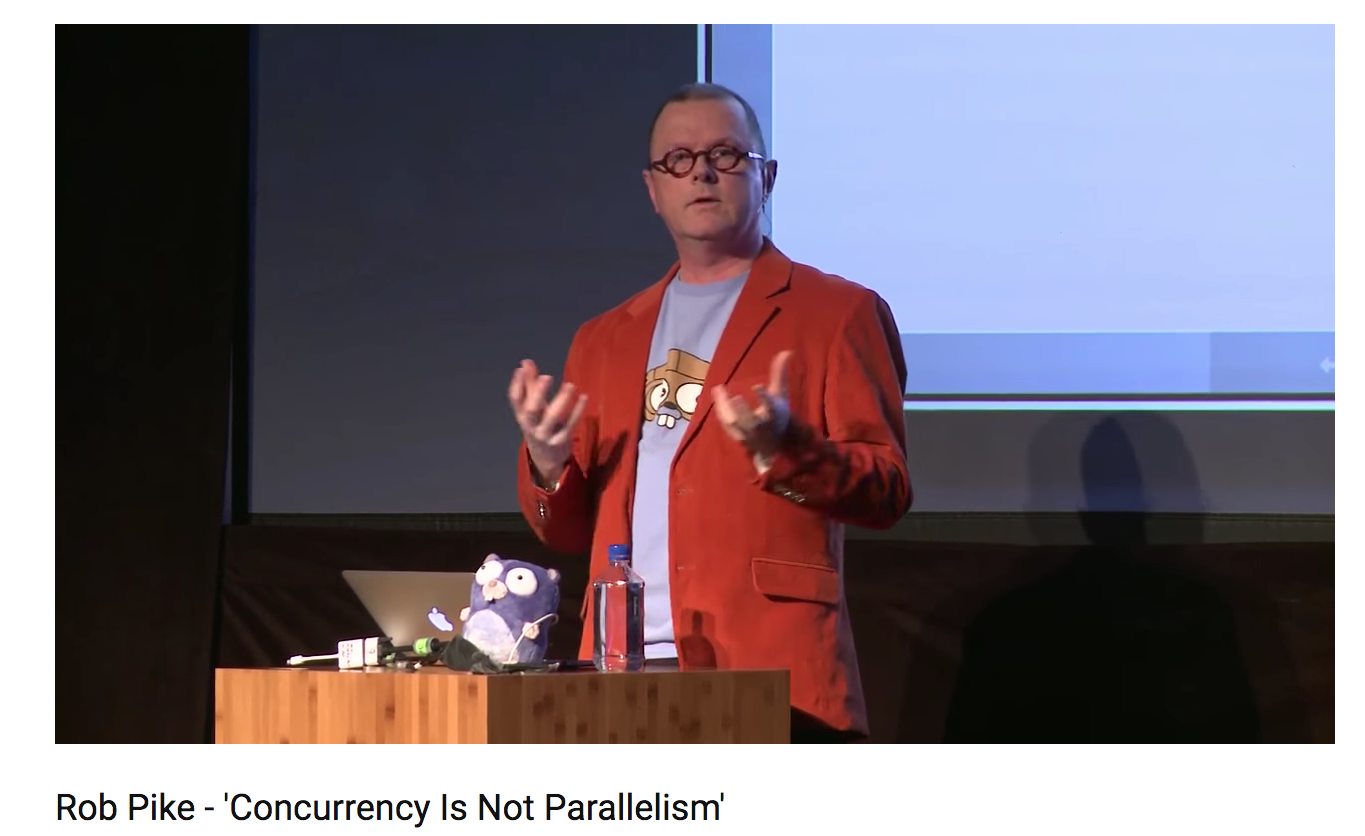
\includegraphics[height=.8\textheight]{rob_talk}
		\caption{\url{https://www.youtube.com/watch?v=cN_DpYBzKso&t=1061s}}
	\end{figure}
\end{frame}

\begin{frame}[fragile]
	\begin{figure}
		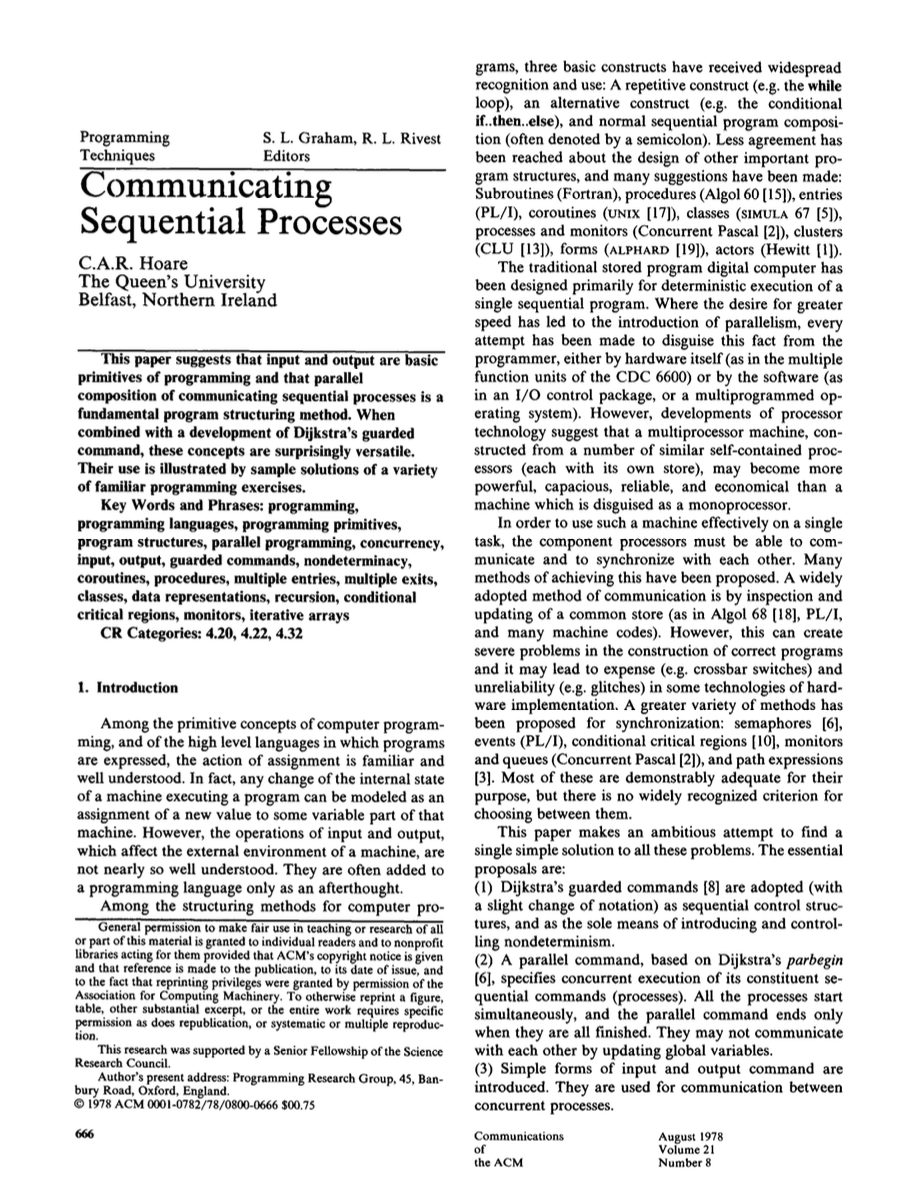
\includegraphics[height=.8\textheight]{tony}
		\caption{Tony Hoare's seminal paper}
	\end{figure}
\end{frame}
\begin{frame}[fragile]
``The most obvious application of the new ideas is to the specification, design,
and implementation of computer systems which continuously act and
interact with their environment. The basic idea is that these systems can be
readily decomposed into subsystems which operate concurrently and interact
with each other as well as with their common environment. The parallel composition
of subsystems is as simple as the sequential composition of lines or
statements in a conventional programming language.``

	Tony Hoare (CSP book, 2015)
\end{frame}





\begin{frame}[fragile]
\begin{lstlisting}[language=Kotlin, basicstyle=\ttfamily]
class PresenterWithDebouncer(
        private val base: Contract.Presenter
) : Contract.Presenter by base {

    override fun onRefresh() {
        base.onRefresh() // HOW ??
    }
}
\end{lstlisting}
\end{frame}


\begin{frame}[fragile]
\begin{lstlisting}[language=Kotlin, basicstyle=\ttfamily]
class Test {

  @Mock
  lateinit var useCase : UseCase

  lateinit var presenter : Contract.Presenter

  @Before
  fun setup() {
      presenter = Presenter(useCase,
              Dispatchers.Unconfined,
              Dispatchers.Unconfined
             )
  }
}
\end{lstlisting}
\end{frame}

\begin{frame}[fragile]
\begin{lstlisting}[language=Kotlin, basicstyle=\ttfamily]
interface Contract {

    interface Presenter {
        suspend fun onRefresh()

        fun bind(view: View)
        fun unbind()
    }

}
\end{lstlisting}
\end{frame}
\begin{frame}[fragile]
\begin{lstlisting}[language=Kotlin, basicstyle=\ttfamily]
class SomeFragment : Fragment(), Contract.View {
  // ...

  override fun showA() = launch(ui){/* ... */}
  override fun hideA() = launch(ui){/* ... */}
  override fun showB() = launch(ui){/* ... */}
  override fun hideB() = launch(ui){/* ... */}
  override fun showC() = launch(ui){/* ... */}
  override fun hideC() = launch(ui){/* ... */}
}
\end{lstlisting}
\end{frame}

\begin{frame}[fragile]
\begin{lstlisting}[language=Kotlin, basicstyle=\ttfamily]
class SomeFragment : Fragment(), Contract.View {
  // ...

  override fun onViewCreated(view: View, 
            savedInstanceState: Bundle?) {
    swipeRefresh.setOnRefreshListener { 
       launch(io){presenter.refresh()}
    }
  }
}
\end{lstlisting}
\end{frame}


\section{Before structured concurrency}

\begin{frame}[fragile]
\begin{lstlisting}[language=Kotlin, basicstyle=\ttfamily]
class Presenter( /*...*/ ) : Contract.Presenter {

  private var view: Contract.View? = null
  private val jobs = mutableListOf<Job>()

  override fun onRefresh() {
    jobs += launch(ui) {/*...*/}
  }
  override fun unbind() {
    view = null
    jobs.forEach { it.cancel() } 
    jobs.clear() 
  }
}
\end{lstlisting}
\end{frame}



\begin{frame}[fragile]
\begin{lstlisting}[language=Kotlin, basicstyle=\ttfamily]
class Presenter(
  private val useCase: UseCase,
  private val ui: Scheduler,
  private val io: Scheduler
) : Contract.Presenter {

  private val bag = CompositeDisposable()

  override fun onRefresh() {
    bag.add(
      useCase
        .observeOn( /*...*/ )
        .subscribeOn( /*...*/ )
        .subscribe { /* ... */ }
    )
  }
}
\end{lstlisting}
\end{frame}




\begin{frame}[fragile]
\begin{lstlisting}[language=Kotlin, basicstyle=\ttfamily]
class Presenter(
  private val useCase: UseCase,
  private val ui: Scheduler,
  private val io: Scheduler
) : Contract.Presenter {

  private val bag = CompositeDisposable()

  override fun unbind() {
    view = null
    bag.clear() // not dispose!
  }
}
\end{lstlisting}
\end{frame}

\begin{frame}[fragile]
	\begin{alertblock}{Question}
Why disposing?
\end{alertblock}
\end{frame}

\begin{frame}[fragile]
\begin{lstlisting}[language=Kotlin, basicstyle=\ttfamily]
class Presenter( /*...*/ ) : Contract.Presenter {

  private var view: Contract.View? = null
  private val jobs = mutableListOf<Job>()

  override fun onRefresh() {
    jobs += launch(ui) {/*...*/}
  }
  override fun unbind() {
    view = null
    jobs.forEach { it.cancel() } // release resource 
    jobs.clear() // avoid memory leaks
  }
}
\end{lstlisting}
\end{frame}



\begin{frame}[fragile]
\begin{lstlisting}[language=Kotlin, basicstyle=\ttfamily]
    job.cancel()
\end{lstlisting}
\end{frame}

\begin{frame}[fragile]
\begin{lstlisting}[language=Kotlin, basicstyle=\ttfamily]
    job.cancelAndJoin()
\end{lstlisting}
\end{frame}

\begin{frame}
``A job can be cancelled it at any time with cancel function that forces it to transition to cancelling state immediately. The job becomes cancelled when it finishes executing it work.''
\end{frame}

\begin{frame}
	\begin{figure}
		\centering
		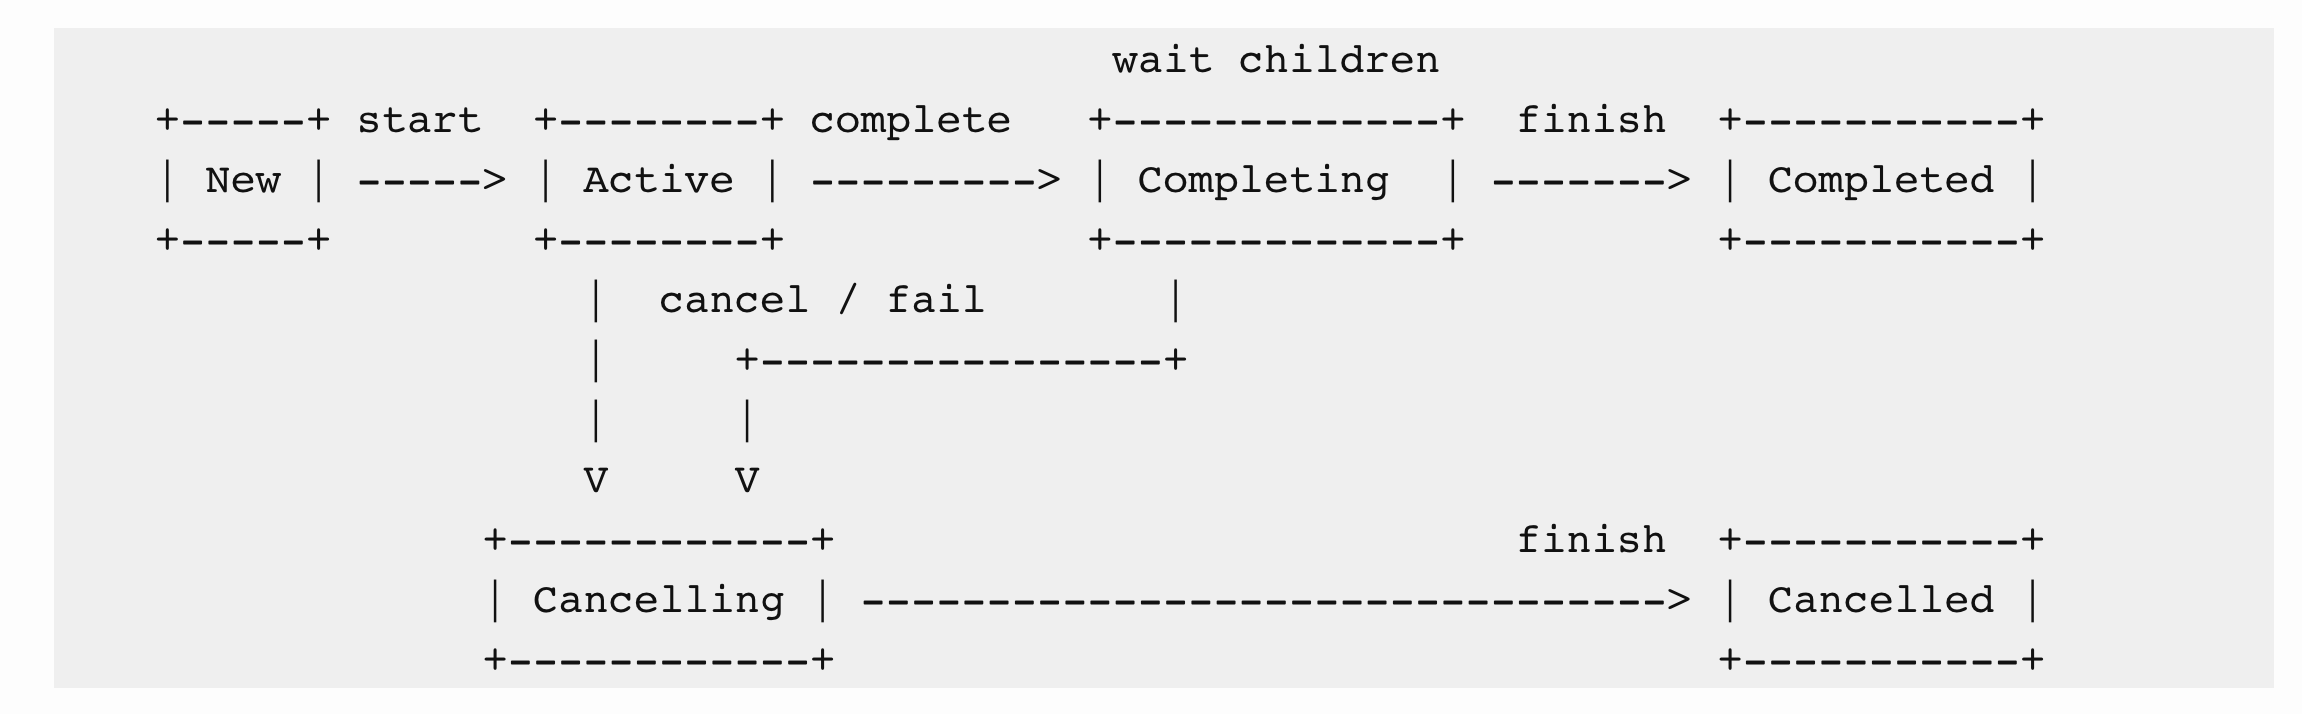
\includegraphics[width=.9\textwidth]{job_cancelling}
	\end{figure}
\url{https://kotlin.github.io/kotlinx.coroutines/kotlinx-coroutines-core/kotlinx.coroutines/-job/index.html}
\end{frame}



\begin{frame}[fragile]
	\begin{alertblock}{Question}
Why a list and not only one reference?
\end{alertblock}
\end{frame}
\begin{frame}[fragile]
\begin{lstlisting}[language=Kotlin, basicstyle=\ttfamily]
class Presenter( /*...*/ ) : Contract.Presenter {

  private var view: Contract.View? = null
  private val jobs = mutableListOf<Job>()

  override fun onA(){ jobs += launch(ui){/*...*/}}
  override fun onB(){ jobs += launch(ui){/*...*/}}
  override fun onC(){ jobs += launch(ui){/*...*/}}
  
  override fun unbind() {
    view = null
    jobs.forEach { it.cancel() } 
    jobs.clear() 
  }
}
\end{lstlisting}
\end{frame}

\begin{frame}[fragile]
	\begin{alertblock}{Assumption}
all processes are independent and can run concurrently (otherwise, need to handle concurrency/coordination via channels, actors, etc) 
\end{alertblock}
\end{frame}
\begin{frame}[fragile]
	\begin{alertblock}{Question}
Why is adding to the list manually error prone?
\end{alertblock}
\end{frame}

\begin{frame}[fragile]
\begin{lstlisting}[language=Kotlin, basicstyle=\ttfamily]
class Presenter( /*...*/ ) : Contract.Presenter {

  private var view: Contract.View? = null
  private val jobs = mutableListOf<Job>()

  override fun onA(){ jobs += launch(ui){/*...*/}}
  override fun onB(){ launch(ui){/*leaking*/}}
  override fun onC(){ jobs += launch(ui){/*...*/}}
  
  override fun unbind() {
    view = null
    jobs.forEach { it.cancel() } 
    jobs.clear() 
  }
}
\end{lstlisting}
\end{frame}


\begin{frame}[fragile]
\frametitle{Parallel decomposition}
\begin{lstlisting}[language=Kotlin, basicstyle=\ttfamily]
suspend fun fetch() : List<Model> {

 val deferredA = async{ /* source A */ }
 val deferredB = async{ /* source B */ }
 val deferredC = async{ /* source C */ }

 val modelA = deferredA.await() 
 val modelB = deferredB.await() 
 val modelC = deferredC.await() 
 return modelA + modelB + modelC
}
\end{lstlisting}
\end{frame}


\begin{frame}[fragile]
\begin{lstlisting}[language=Kotlin, basicstyle=\ttfamily]
suspend fun fetch() : List<Model> {

 val deferredA = async{/*long running task*/}
 val deferredB = async{/*quickly throws exception*/}
 val deferredC = async{/*...*/ }

 val modelA = deferredA.await()  // <-- wait A
 val modelB = deferredB.await() 
 val modelC = deferredC.await() 
 return modelA + modelB + modelC
}
\end{lstlisting}
\end{frame}

\section{Welcome structured concurrency}

\begin{frame}[fragile]
\begin{lstlisting}[language=Kotlin, basicstyle=\ttfamily]

val scope : CoroutineScope = /*...*/

fun onRefresh() {
  scope.launch {/*...*/}
}
\end{lstlisting}
\end{frame}

\begin{frame}[fragile]
\begin{lstlisting}[language=Kotlin, basicstyle=\ttfamily]

val scope : CoroutineScope = /*...*/
val dispatcher : CoroutineDispatcher = /*...*/

fun onRefresh() {
  scope.launch(dispatcher){/*...*/}
}
\end{lstlisting}
\end{frame}

\begin{frame}[fragile]
\begin{lstlisting}[language=Kotlin, basicstyle=\ttfamily]

val scope : CoroutineScope = /*...*/
val dispatcher : CoroutineDispatcher = /*...*/

fun CoroutineScope.onRefresh() { // convention 
  launch(dispatcher){/*...*/}
}

\end{lstlisting}
\end{frame}



\begin{frame}[fragile]
\begin{lstlisting}[language=Kotlin, basicstyle=\ttfamily]

val scope : CoroutineScope = /*...*/
val dispatcher : CoroutineDispatcher = /*...*/

fun onRefresh() {
  scope.launch{ // parent 
     launch(dispatcher){ // child 
       /*...*/
     }
  }
}
\end{lstlisting}
\end{frame}

\begin{frame}[fragile]
\begin{lstlisting}[language=Kotlin, basicstyle=\ttfamily]
class Presenter( /*...*/ ) : 
      Contract.Presenter, CoroutineScope {

  override fun onRefresh() {
    launch {/*...*/}
  }
}
\end{lstlisting}
\end{frame}

\begin{frame}[fragile]
\begin{lstlisting}[language=Kotlin, basicstyle=\ttfamily]
class Presenter( scope : CoroutineScope) : 
      Contract.Presenter, CoroutineScope by scope {

  override fun onRefresh() {
    launch {/*...*/}
  }
}
\end{lstlisting}
\end{frame}


\begin{frame}[fragile]
\begin{lstlisting}[language=Kotlin, basicstyle=\ttfamily]
class Presenter( /*...*/) : 
          Contract.Presenter, CoroutineScope {

  private lateinit var job : Job
  override val coroutineContext: CoroutineContext
    get() = ui + job

  override fun bind(view : View) {
    job = Job()  
  }

  override fun onRefresh() {
    launch(ui) {/*...*/}
  }
  override fun unbind() {
    job.cancel()
  }
}
\end{lstlisting}
\end{frame}
\begin{frame}[fragile]
\begin{lstlisting}[language=Kotlin, basicstyle=\ttfamily]
class Presenter( /*...*/ ) : Contract.Presenter,
   CorotuineScope {

  override fun onA(){ launch{/*...*/}}
  override fun onB(){ launch{/*...*/}}
  override fun onC(){ launch{/*...*/}}
  
  override fun unbind() {
    job.cancel() 
  }
}
\end{lstlisting}
\end{frame}
\begin{frame}[fragile]
Possible alternatives where to implement CoroutineScope:
\begin{itemize}
\item Activity/fragment/custom view 
\item Lifecycle 
\item Some binder in between 
\end{itemize}
\end{frame}

\begin{frame}[fragile]
Show code samples:
\begin{itemize}
\item Testability 
\item Parallel decomposition example 
\end{itemize}
\end{frame}


\section{Exceptions}

\mycomment{%
\begin{frame}[fragile]
\frametitle{Unchecked exceptions are good}
\begin{lstlisting}[language=Kotlin, basicstyle=\ttfamily]
interface ApiService {

    @GET("/v1/api/item")
    suspend fun fetch() : ApiResponse
}
\end{lstlisting}
\end{frame}

\begin{frame}[fragile]
\frametitle{Unchecked exceptions are good}
\begin{lstlisting}[language=Kotlin, basicstyle=\ttfamily]
interface UseCase {
    suspend fun fetch() : Model
}

class UseCaseAPi(private val apiService: ApiService) : 
       UseCase {
   
  override suspend fun fetch(): Model =
    apiService.fetch().let { map(it) }

  private fun map(apiResponse: ApiResponse) : Model 
     = TODO()
}
\end{lstlisting}
\end{frame}

\begin{frame}[fragile]
\frametitle{Unchecked exceptions are good}
\begin{lstlisting}[language=Kotlin, basicstyle=\ttfamily]
override fun onRefresh() {
     fetch()
}

fun CoroutineScope.fetch() {
  launch(io) {
    val model = useCase.fetch()
      render(model)
    }
  }

fun CoroutineScope.render(model : Model) {
  launch(ui) {
    view?.show(model)
  }
}
\end{lstlisting}
\end{frame}

\begin{frame}[fragile]
\frametitle{Unchecked exceptions are good}
\begin{lstlisting}[language=Kotlin, basicstyle=\ttfamily]
\end{lstlisting}
\end{frame}


\begin{frame}[fragile]
\frametitle{Unchecked exceptions are good}
\begin{lstlisting}[language=Kotlin, basicstyle=\ttfamily]
\end{lstlisting}
\end{frame}


\begin{frame}[fragile]
\frametitle{Unchecked exceptions are bad}
\begin{lstlisting}[language=Kotlin, basicstyle=\ttfamily]
\end{lstlisting}
\end{frame}

\begin{frame}[fragile]
\frametitle{Antipatterns}
\begin{lstlisting}[language=Kotlin, basicstyle=\ttfamily]
\end{lstlisting}
\end{frame}

\begin{frame}[fragile]
\frametitle{Checked exceptions are good}
\begin{lstlisting}[language=Kotlin, basicstyle=\ttfamily]
\end{lstlisting}
\end{frame}

\begin{frame}[fragile]
\frametitle{Checked exceptions are bad}
\begin{lstlisting}[language=Kotlin, basicstyle=\ttfamily]
\end{lstlisting}
\end{frame}

\begin{frame}[fragile]
Kotlin does not support for this reason check exceptions 
\begin{lstlisting}[language=Kotlin, basicstyle=\ttfamily]
\end{lstlisting}
\end{frame}
}




\begin{frame}[fragile]
General questions:
\begin{itemize}
\item Why unchecked exceptions are good?
\item Why unchecked exceptions are bad?
\item Why checked exceptions are good?
\item Why checked exceptions are bad?
\item Alternatives?
\end{itemize}
How does this apply to coroutines and structured concurrency?
\end{frame}

\begin{frame}[fragile]
\begin{lstlisting}[language=Kotlin, basicstyle=\ttfamily]
private fun CoroutineScope.fetch() = launch (ui) {
  try {
    val items = async(io){ usecase.fetch() }
              .await() 
    view?.let {
      it.showResults(items)
    }
  } catch (e: Exception) {
      view?.showError(e.localizedMessage)
  } finally {
      view?.hideLoading()
  }
}
\end{lstlisting}
\end{frame}
\begin{frame}[fragile]
\begin{lstlisting}[language=Kotlin, basicstyle=\ttfamily]
private fun CoroutineScope.fetch() = launch (ui) {
  try {
    val items = withContext(io){ usecase.fetch() }
    view?.let {
      it.showResults(items)
    }
  } catch (e: Exception) {
      view?.showError(e.localizedMessage)
  } finally {
      view?.hideLoading()
  }
}
\end{lstlisting}
\end{frame}


\begin{frame}[fragile]
What about algebraic data types and parallel decomposition?
\end{frame}


\begin{frame}[fragile]
\frametitle{Embrace concurrency}
Mobile environment is intrinsically concurrent.

Concurrency abstractions available in Kotlin:
\begin{itemize}
\item Parallel decomposition via async/await 
\item Channels/CSP 
\item Actors
\end{itemize}


\end{frame}
\begin{frame}[fragile]
Notice that in Kotlin 1.3.11/coroutines 1.0.1 both channels and actors are still experimental.

Channels API likely to be changed to support
\begin{itemize}
\item cold channels 
\item structured concurrency 
\end{itemize}
\end{frame}

\begin{frame}[fragile]
There is much more about structured concurrency:
\begin{itemize}
\item SupervisorJob
\item cancelChildren() vs cancel
\item github issues about exception handling 
\end{itemize}
\end{frame}



\begin{frame}{References}
		\begin{itemize}
			\item Structured Concurrency - R. Elizarov
				\begin{itemize}
					\item \url{https://medium.com/@elizarov/structured-concurrency-722d765aa952}
				\end{itemize}
			\item Explicit Concurrency - R. Elizarov
				\begin{itemize}
					\item \url{https://medium.com/@elizarov/explicit-concurrency-67a8e8fd9b25}
				\end{itemize}
			\item Blocking threads, suspending coroutines - R. Elizarov 
			\begin{itemize}
					\item \url{https://medium.com/@elizarov/blocking-threads-suspending-coroutines-d33e11bf4761}
				\end{itemize}
			\item Kotlin Coroutines in Practice - R. Elizarov 
			\begin{itemize}
					\item \url{https://www.youtube.com/watch?v=a3agLJQ6vt8}
				\end{itemize}
			\item Guide to kotlinx.coroutines by example 
				\begin{itemize}
					\item \url{https://github.com/Kotlin/kotlinx.coroutines/blob/master/coroutines-guide.md}
				\end{itemize}
		\end{itemize}
	\end{frame}

\begin{frame}{Github}
		\begin{itemize}
			\item Integrate ticker channels into structured concurrency
				\begin{itemize}
					\item \url{https://github.com/Kotlin/kotlinx.coroutines/issues/540}
				\end{itemize}
			\item Async builder and cancellation in structured concurrency				\begin{itemize}
					\item \url{https://github.com/Kotlin/kotlinx.coroutines/issues/763}
				\end{itemize}
			\item Global handler for fatal errors in coroutine machinery			\begin{itemize}
					\item \url{https://github.com/Kotlin/kotlinx.coroutines/issues/808}
				\end{itemize}
		\end{itemize}
	\end{frame}






\plain{Questions?}

\end{document}

\begin{frame}[fragile]
\begin{lstlisting}[language=Kotlin, basicstyle=\ttfamily]
\end{lstlisting}
\end{frame}


\plain{Questions?}

%\begin{frame}[allowframebreaks] {References}
% \bibliography{demo}
% \bibliographystyle{abbrv}
%\end{frame}

\end{document}
\begin{lstlisting}[language=Kotlin, basicstyle=\ttfamily]
\end{lstlisting}

\begin{frame}
\begin{lstlisting}[language=Kotlin, basicstyle=\ttfamily]
\end{lstlisting}
\end{frame}
